\documentclass[../main.tex]{subfiles}
\begin{document}
\chapter{Basics Of Vectors}
\section{Definition and Axioms}
\subsection{Introductory Definitions}
A vector is specified by a (positive) magnitude and a direction in space.
We can represent a vector as line segment between two points $A$ and $B$, $\vec{v} = \avec{AB}$.
$\vec{v}$ has length $|\vec{v}|$ and direction from $A$ to $B$.
If we chose an origin $O$ then considering a point $A$ it has position vector denoted $\vec{a} = \avec{OA}$.
\begin{definition}[Vector Space]
  A \textit{vector space}, $V$, over $\R$ or $\C$ is a collection of vectors $\vec{v} \in V$, together with two operations:
  \begin{enumerate}
    \item Addition of two vectors
    \item Multiplication by a scalar (from $\R$ or $\C$ respectively)
  \end{enumerate}
\end{definition}
Vector addition has to satisfy the following axioms:
\begin{enumerate}
  \item \textbf{Commutativity -} $\vec{a} + \vec{b} = \vec{b} + \vec{a}$
  \item \textbf{Associativity -} $(\vec{a} + \vec{b}) + \vec{c} = \vec{a} + (\vec{b} + \vec{c})$
  \item \textbf{Identity -} There exists a vector $\vec{0}$ such that for all $a \in V$, $\vec{a} + \vec{0} = \vec{a}$
  \item \textbf{Inverse -} For all vectors $\vec{a} \in V$, there is a vector ($-\vec{a}$) such that $\vec{a} + (-\vec{a}) = \vec{0}$.
\end{enumerate}
Scalar multiplication has to satisfy the following axioms (Where $\lambda$ and $\mu$ are scalars):
\begin{enumerate}
  \item $\lambda(\vec{a} + \vec{b}) = \lambda \vec{a} + \lambda \vec{b}$
  \item $(\lambda + \mu)\vec{a} = \lambda \vec{a} + \mu \vec{a}$
  \item $\lambda(\mu \vec{a}) = (\lambda \mu)\vec{a}$
  \item $1(\vec{a}) = \vec{a}$
\end{enumerate}
\begin{remark}
  Vectors under addition are an abelian group.
\end{remark}
\begin{remark}[Warning]
  $\R^{n}$ is a vector space with addition (component-wise) and scalar multiplication.
  We can represent $\R$ by a line and this could make us think that any line is a vector space however this is not true as the space does not necessarily contain $O$.
  E.g. $x + y = d$ is not a vector space.
\end{remark}

\subsection{Geometric View}
Given vectors $\vec{a}$ and $\vec{b}$ which are the position vectors of $A$ and $B$ respectively, we can construct the parallelogram $OACB$:
\begin{center}
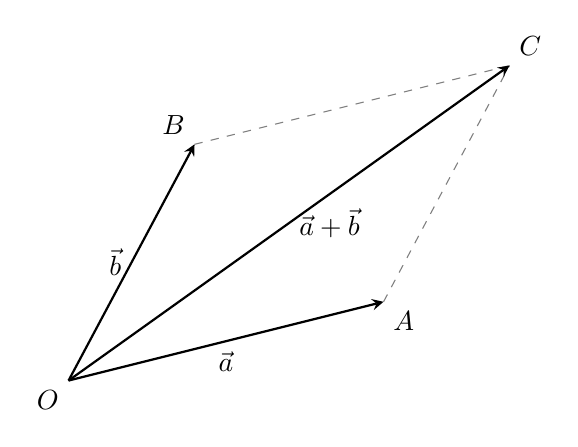
\begin{tikzpicture}[scale=2,>=stealth]
  \coordinate (O) at (0,0);
  \coordinate (A) at (2,0.5);   % vector a
  \coordinate (B) at (0.8,1.5); % vector b
  \coordinate (C) at (2.8,2);   % a + b

  \node[below left] at (O) {$O$};
  \node[below right] at (A) {$A$};
  \node[above left] at (B) {$B$};
  \node[above right] at (C) {$C$};

  \draw[->, thick, black] (O) -- (A) node[midway, below] {$\vec{a}$};
  \draw[->, thick, black] (O) -- (B) node[midway, left] {$\vec{b}$};

  \draw[dashed, gray] (A) -- (C);
  \draw[dashed, gray] (B) -- (C);

  \draw[->, thick, black] (O) -- (C) node[midway, right] {$\vec{a} + \vec{b}$};
\end{tikzpicture}
\end{center}

and then $\vec{a} + \vec{b} = \vec{c}$, where $\vec{c}$ is the position vector of $C$.

Given a vector $\vec{a}$ which is the position vector of a point $A$ and a $\lambda \in \R$.
$\lambda \vec{a}$ is a position vector of a point on the line through $OA$, with length $|\lambda \vec{a}| = |\lambda||\vec{a}$.

\begin{center}
\begin{tikzpicture}[scale=2,>=stealth]
  \coordinate (O) at (0,0);
  \coordinate (A) at (1.2,0.6);
  \coordinate (B) at (2.4,1.2);
  \coordinate (C) at (-1.2,-0.6);

  % Guide line
  \draw[dashed, gray] (-1.6,-0.8) -- (3,1.5);

  % Original vector
  \draw[->, thick, black] (O) -- (A) node[midway, below right] {$\vec{a}$};

  % Scaled vector
  \draw[->, black] (O) -- (B) node[near end, below right] {$\lambda \vec{a}$};

  % Reversed vector
  \draw[->, black] (O) -- (C) node[near end, below right] {$-\frac{\lambda}{2} \vec{a}$};

  % Label points
  \fill (O) circle (0.03);
  \node[below right] at (O) {$O$};
  \node[below right] at (A) {$A$};
\end{tikzpicture}
\end{center}
\begin{remark}[Note]
  $\{\lambda \vec{a}: \lambda \in \R\}$ is the set of all points on the line through $OA$.
\end{remark}

\subsection{Linear Combination and Span}
\begin{definition}[Linear Combination]
  Given $n$ vectors $\vec{r}_1, \vec{r}_2, \ldots, \vec{r}_n$, a \textit{linear combination} of those vectors is a vector of the form:
  \[
    \sum_{i = 1}^{n} \lambda_i \vec{r}_i  = \lambda_1 \vec{r}_1 + \lambda_2 \vec{r}_2 + \cdots + \lambda_n \vec{r}_n
  \]
  where $\lambda_1, \lambda_2, \ldots, \lambda_n$ are scalars.
\end{definition}
We can also define the ``space'' of all linear combinations of a set of vectors:
\begin{definition}[Span]
  Given $n$ vectors $\vec{r}_1, \vec{r}_2, \ldots, \vec{r}_n$, their \textit{span} is the set of all linear combinations of those vectors.
  \[
    \Span\{\vec{r}_1, \vec{r}_2, \ldots, \vec{r}_n\} = \left\{\sum_{i = 1}^{n} \lambda_i \vec{r}_i : \lambda_i \in K\right\}
  \]
  where $K$ is either $\C$ or $\R$ depending on the vector space.
\end{definition}
\begin{definition}[Parallel]
  Any two vectors $\vec{a}$ and $\vec{b}$ are \textit{parallel} if $\vec{a} = \lambda \vec{b}$ or $\vec{b} = \lambda \vec{a}$ for some $\lambda \in \R$.
  We denote this $\vec{a} \parallel \vec{b}$.
\end{definition}
\begin{remark}[Note]
  Since we allow $\lambda = 0$, $\vec{0} \parallel \vec{a}$ for any $\vec{a}$.
\end{remark}
If $\vec{a} \centernot\parallel \vec{b}$ ($\vec{a}$ and $\vec{b}$ are not parallel), then $\Span\{\vec{a}, \vec{b}\}$ is a plane through $O$, $A$, and $B$.
\begin{definition}[Unit Vector]
  A \textit{unit vector} is a vector with length $1$.
  They are denoted $\uvec{v}$.
\end{definition}
\section{Scalar Product}
The \textit{scalar product} of two vectors within a vector space returns a scalar (either real or complex).
\subsection{Geometric Viewpoint in \texorpdfstring{$\R^{n}$}{Real Vector Spaces}}
First consider the usual scalar product in $\R^{n}$.
\begin{definition}[Scalar Product]
  The \textit{scalar product} of two vectors $\vec{a}$ and $\vec{b}$ is defined as:
  \[
    \vec{a} \cdot \vec{b} = |\vec{a}||\vec{b}|\cos\theta
  \]
  where $\theta$ is the angle between $\vec{a}$ and $\vec{b}$.
\end{definition}
\begin{remark}[Note]
  If $|\vec{a}| = 0$ or $|\vec{b}| = 0$ then $\theta$ is not well defined, but in that case we have $\vec{a} \cdot \vec{b} = 0$.
\end{remark}
Intuitively the dot product is the product of the parts of $\vec{a}$ and $\vec{b}$ that are parallel.

The scalar product in $\R^{n}$ satisfies the following properties:
\begin{enumerate}
  \item $\vec{a} \cdot \vec{b} = \vec{b} \cdot \vec{a}$
  \item $\vec{a} \cdot \vec{a} = |\vec{a}|^2 \geq 0$ (and $|\vec{a}| = 0 \iff \vec{a} = \vec{0}$)
  \item $(\lambda \vec{a}) \cdot \vec{b} = \lambda (\vec{a} \cdot \vec{b}) = \vec{a} \cdot (\lambda \vec{b})$
  \item $\vec{a} \cdot (\vec{b} + \vec{c}) = \vec{a} \cdot \vec{b} + \vec{a} \cdot \vec{c}$
\end{enumerate}
\begin{definition}[Orthogonal]
  Any two vectors $\vec{a}$ and $\vec{b}$ are \textit{orthogonal} or \textit{perpendicular} if $\vec{a} \cdot \vec{b} = 0$.
  We denote this $\vec{a} \perp \vec{b}$.
\end{definition}
\begin{remark}[Note]
  We also also allow $\vec{a} = \vec{0}$ or $\vec{b} = \vec{0}$ and hence $\vec{0}$ is orthogonal to any other vector.
\end{remark}
\begin{definition}[Projection]
  Given two vectors $\vec{a}$ and $\vec{b}$, the projection of $\vec{b}$ onto $\vec{a}$ is:
  \[
    \uvec{a}|\vec{b}|\cos \theta = (\uvec{a} \cdot \vec{b}) \uvec{a}
  \]
\end{definition}

\begin{center}
\begin{tikzpicture}[scale=2,>=stealth]
  \coordinate (O) at (0,0);
  \coordinate (A) at (2,0);
  \coordinate (B) at (1.2,1.4);
  \coordinate (P) at (1.2,0);

  % vectors a and b
  \draw[->, black] (O) -- (A) node[near end, below] {$\vec{a}$};
  \draw[->, black] (O) -- (B) node[midway, left] {$\vec{b}$};

  % projection line
  \draw[dashed, gray] (B) -- (P);

  % projection of b onto a
  \draw[->, thick, black] (O) -- (P) node[midway, below] {$\underbrace{(|\vec{b}|\cos\theta)\uvec{a}}_{\text{projection of $\vec{b}$ onto $\vec{a}$}}$};

  % angles
  \draw (0.5,0) arc[start angle=0, end angle=49, radius=0.5];
  \node at (0.6,0.2) {$\theta$};
  \draw ($(P)+(0,0.1)$) -- ($(P)+(0.1,0.1)$) -- ($(P)+(0.1,0)$);
\end{tikzpicture}
\end{center}
We can use the scalar product to quickly derive the cosine rule:
\begin{proof}
  \begin{align*}
    |\avec{BC}|^2 &= |\avec{AC} - \avec{AB}|^2 \\
                  &= (\avec{AC} - \avec{AB}) \cdot (\avec{AC} - \avec{AB}) \\
                  &= |\avec{AC}|^2 - 2 \avec{AB} \cdot \avec{AC} + |\avec{AB}|^2 \\
                  &= |\avec{AC}|^2 + |\avec{AB}|^2 - 2 |\avec{AB}||\avec{AC}|\cos\theta
  \end{align*}
\end{proof}
\subsection{General Algebraic Viewpoint}
This definition generalises to any other vector space, keeping the same axioms.
\begin{definition}[Inner/Scalar Product]
  In a real vector space $V$, an \textit{inner product} or \textit{scalar product} is a map $V \times V \to \R$ that satisfies:
  \begin{enumerate}
    \item \textbf{Symmetry -} $\vec{x} \cdot \vec{y} = \vec{y} \cdot \vec{x}$
    \item \textbf{Linearity in 2nd Argument -} $\vec{x} \cdot(\lambda \vec{y} + \mu \vec{z}) = \lambda \vec{x} \cdot \vec{y} + \mu \vec{x} \cdot \vec{z}$
    \item \textbf{Positive Definiteness - } $\vec{x} \cdot \vec{x} \geq 0$ with equality if and only if $\vec{x} = \vec{0}$
  \end{enumerate}
  We denote it either $\vec{x} \cdot \vec{y}$ or $\inner{\vec{x}}{\vec{y}}$.
\end{definition}
\begin{remark}[Note]
  We get linearity in the first argument also because of symmetry.
\end{remark}
\begin{definition}[Norm]
  The norm of a vector $\vec{a}$ is given by $\sqrt{\vec{a} \cdot \vec{a}}$.
  We denote this as either $|\vec{a}|$ or $\norm{\vec{a}}$.
\end{definition}
\end{document}
